\documentclass[a4paper]{article}
\usepackage[utf8]{inputenc}
\usepackage{fancyhdr}
\usepackage[margin=2.5cm]{geometry}
\usepackage{amsmath, amssymb}
\usepackage{aligned-overset}


% eigene commands
\newcommand{\epszero}{\epsilon_0}
% partielle ableitungen in Kugelkoordinaten
\newcommand{\delr}{\partial_r}
\newcommand{\delp}{\partial_\phi}
\newcommand{\delt}{\partial_\theta}
% einheisvektoren in kugelkoordinaten
\newcommand{\er}{\hat{e}_r}
\newcommand{\et}{\hat{e}_\theta}
\newcommand{\ep}{\hat{e}_\phi}
% 1/4piepsilon0
\newcommand{\kco}{\frac{1}{4\pi\epsilon_0}}

\fancyhf{}
% vspaces in den headern fuer Distanzen notwendig
% linke Seite: Namen der Abgabegruppe
\lhead{\textbf{Etem Kalyon\\Matthias Maile\\Roman Surma}\vspace{1.5cm}}
% rechte Seite: Modul, Gruppe, Semester
\rhead{\textbf{Physik II - Gruppe 2\\Sommersemester 2020}\vspace{1.5cm}}
% Center: nr. des blattes
\chead{\vspace{2.5cm}\huge{\textbf{1. Übungsblatt}}}
% benoetigt damit der eigentliche Text nicht in der Überschrift steckt
\setlength{\headheight}{4cm} 

\usepackage{graphicx}

\begin{document}
% pagestyle nicht global festgelegt, da sonst bei allen Seiten Überschrift ist
% daher muss hier fancy aktiviert werden (für eine Seite, daher thispagestyle)
\thispagestyle{fancy}

\section*{Aufgabe 1}
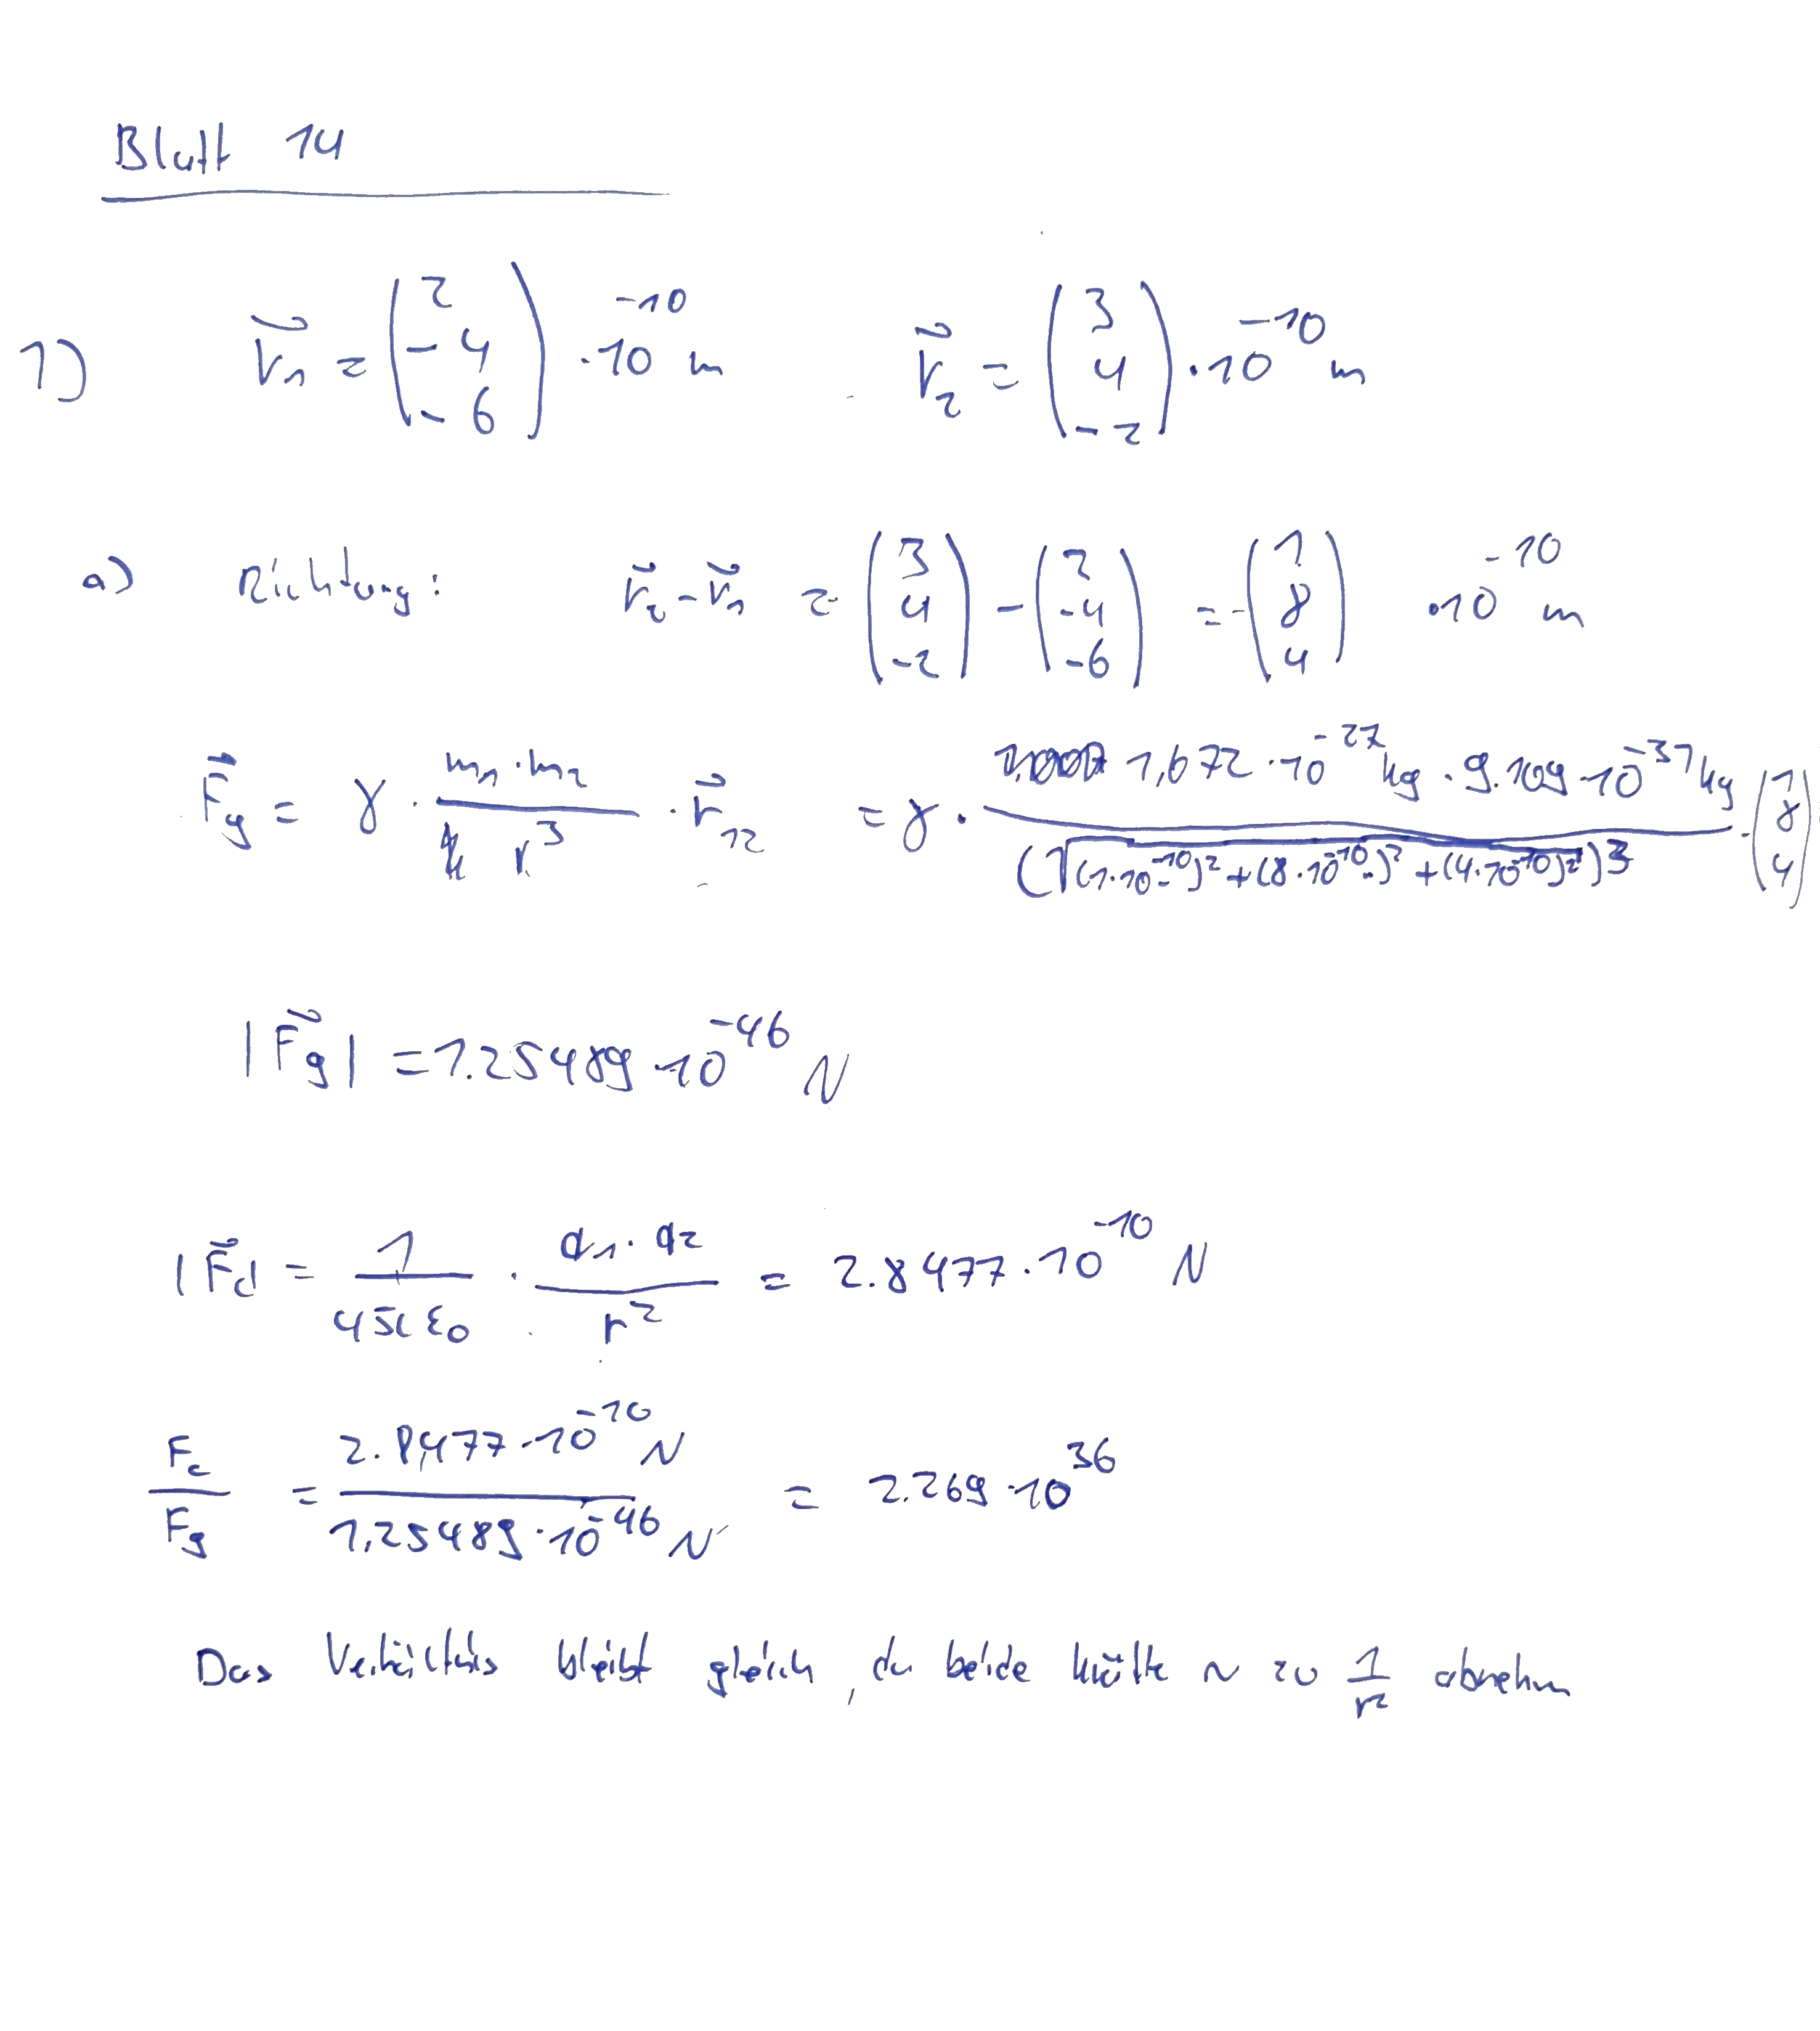
\includegraphics[width=15cm]{1.jpg}

\newpage
\setlength{\headheight}{0cm}
\section*{Aufgabe 2}
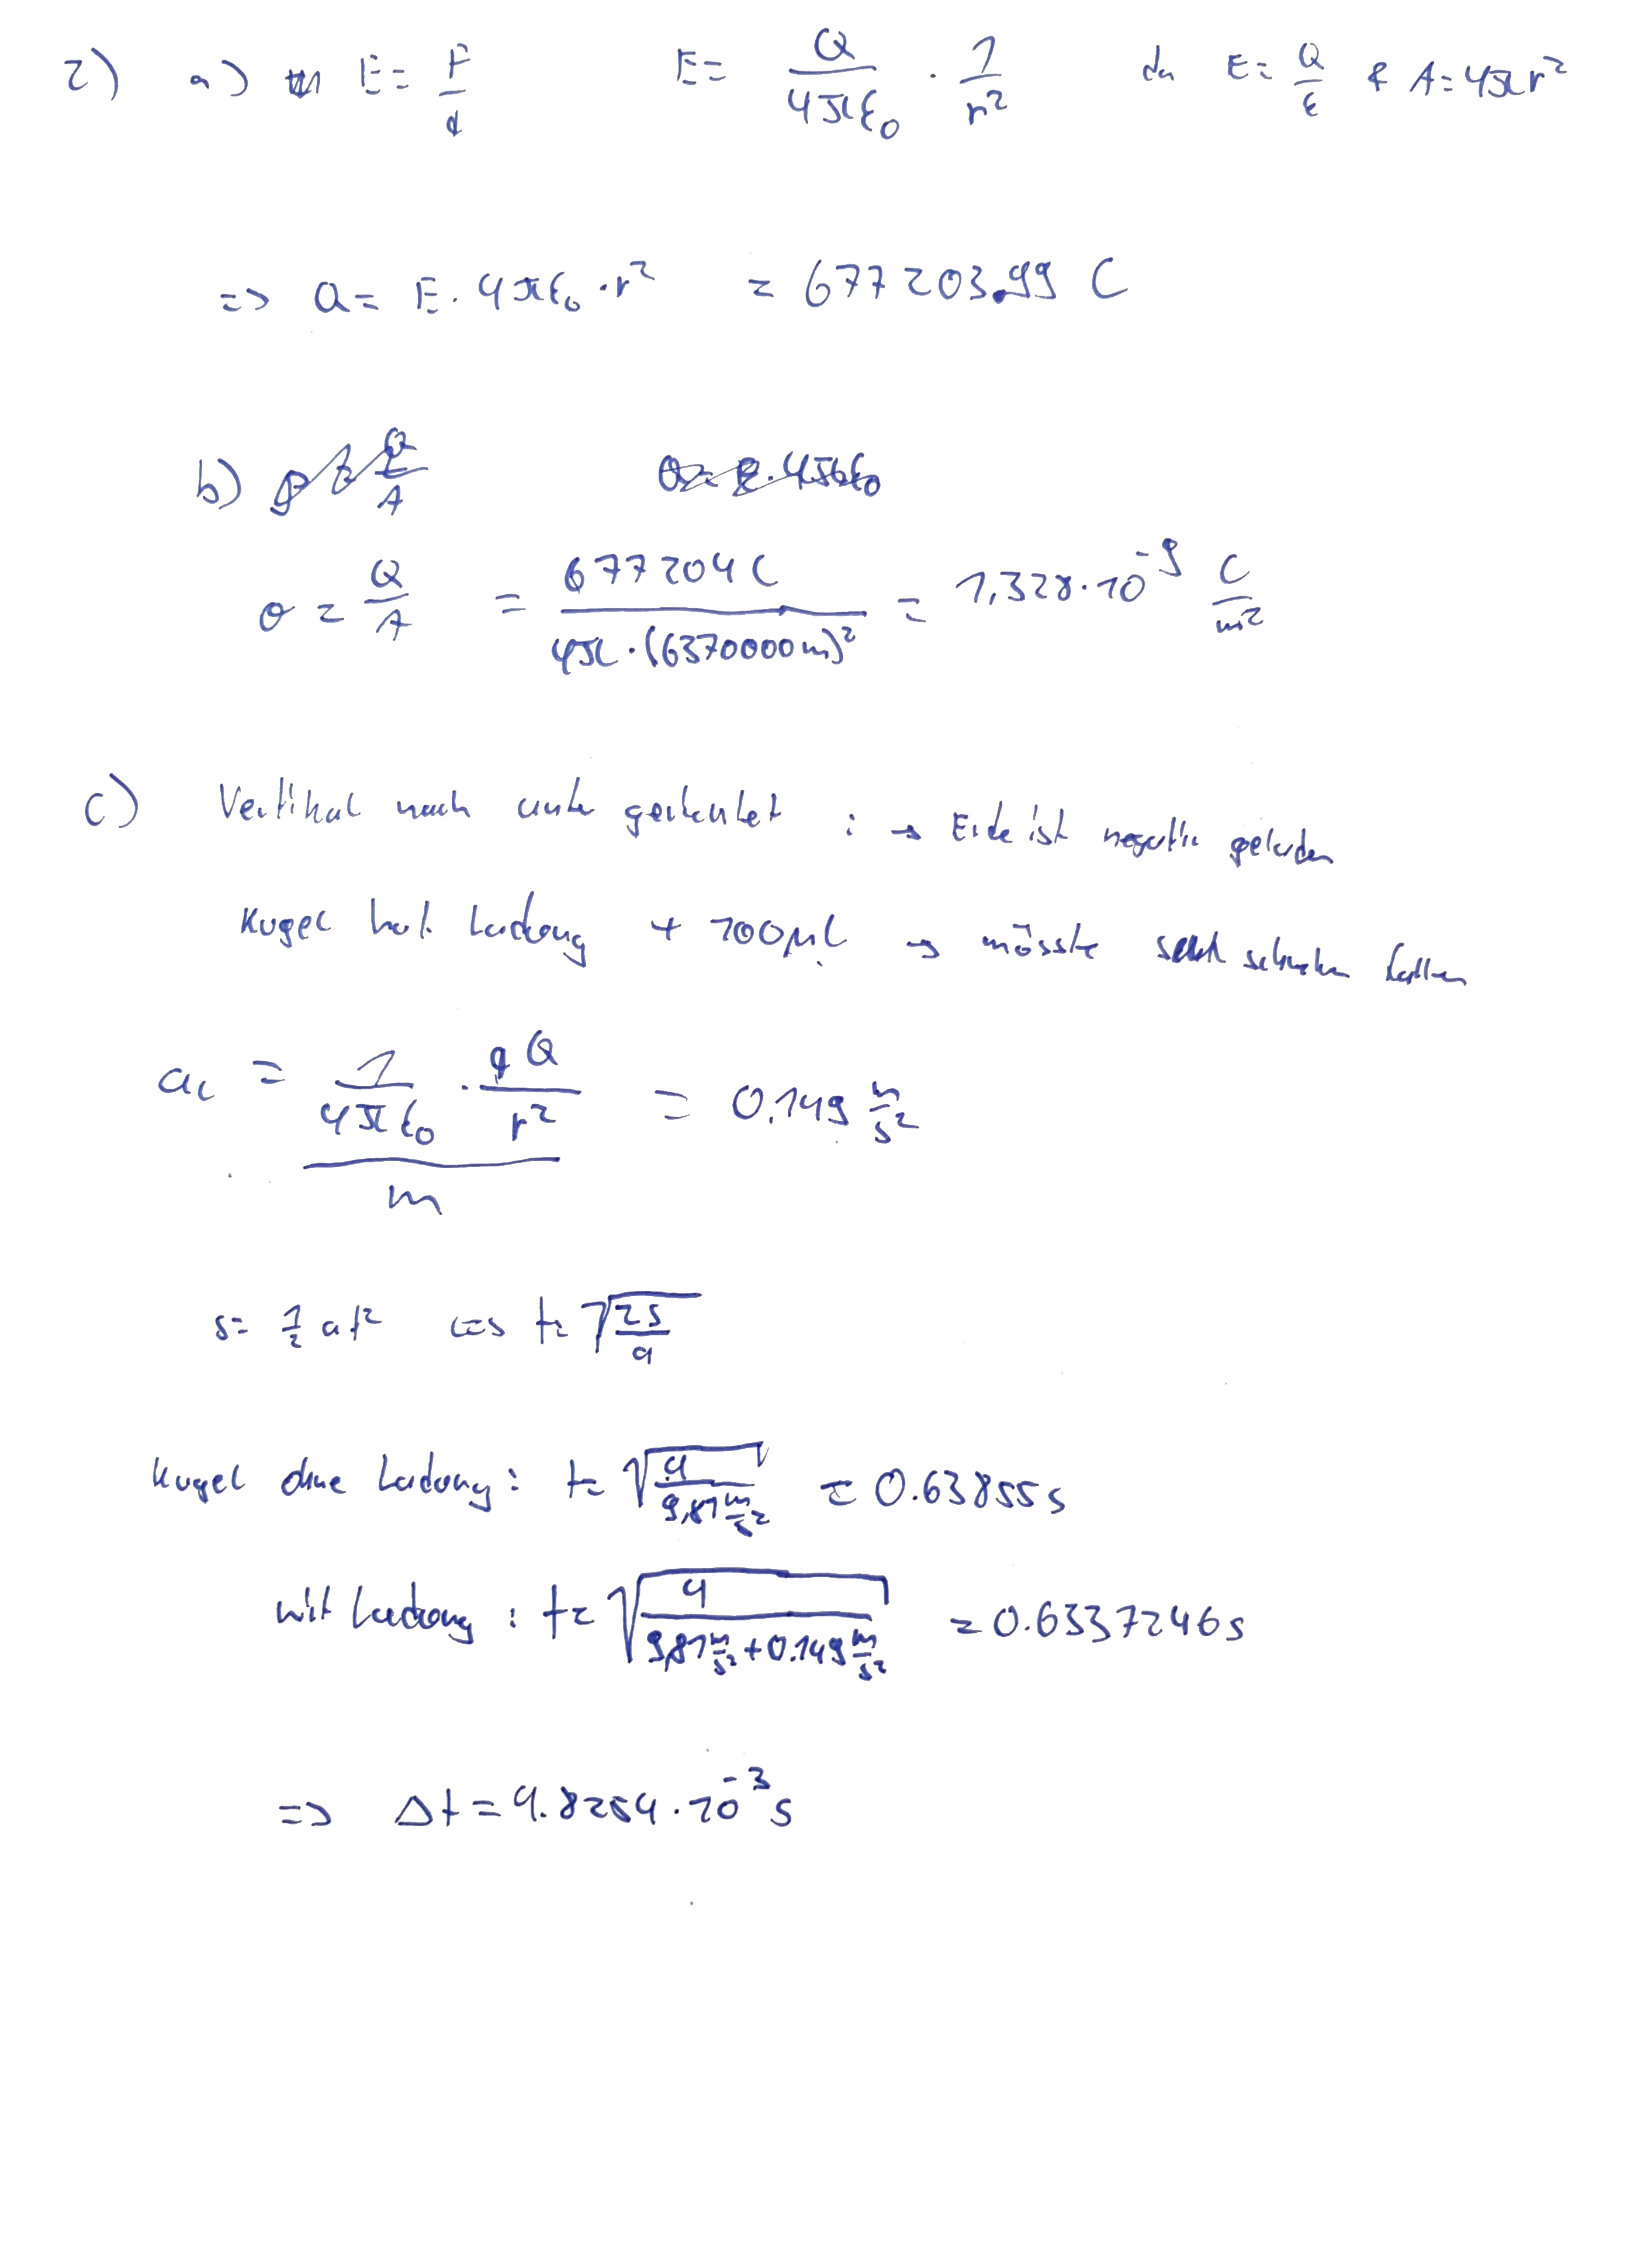
\includegraphics[width=15cm]{2.jpg}

\newpage
\section*{Aufgabe 3}
% ...
Die Coulomb- und die Gewichtskraft sind definiert als:
\[
	F_C = \kco \frac{q_1q_2}{r^2} \qquad F_G = m*g
\]
Wir definieren $q_3 = \frac{q_1 + q_2}{2} $, die Ladung  beider Kugeln nach dem Ladungsausgleich. Aus den trigonometrischen Identitäten folgt das Verhältniss von $F_C$ und $F_G$:
\begin{align*}
	\tan \theta &= \frac{F_C}{F_G} =  \kco \frac{q_1q_2}{mg \cdot r^2}
\end{align*}
Für $\theta_2$ lässt sich die das Verhältniss von $q_1$ und $q_2$ herleiten:
\begin{align*}
	\tan \theta_2 &= \kco \frac{q_3^2}{mg \cdot r_2^2} \\
	\Leftrightarrow
	q_3^2 &= \tan \theta_2 \cdot mg r_2^2 * 4\pi\epsilon_0 \\
	\Leftrightarrow
	q_3 = \frac{q_1 + q_2}{2} &= \sqrt{\tan \theta_2 \cdot mg r_2^2 * 4\pi\epsilon_0} \\
	\Leftrightarrow
	q_1 &= \sqrt{\tan \theta_2 \cdot mg r_2^2 * 16\pi\epsilon_0} - q_2 \\
\end{align*}
Aus $\theta_1$ folgt zuletzt:
\begin{align*}
	\tan \theta_1 &= \kco \frac{q_1q_2}{mg \cdot r_1^2} \\
	\tan \theta_1 &= \kco \frac{ \left( \sqrt{\tan \theta_2 \cdot mg r_2^2 * 16\pi\epsilon_0} - q_2 \right) q_2}{mg \cdot r_1^2} \\
	% umstellen fuer pq formel
	0 &= q_2^2 - q_2 \sqrt{\tan \theta_2 \cdot mg r_2^2 * 16\pi\epsilon_0}  + \tan \theta_1 * 4\pi\epsilon_0	*mg r_1^2 
\end{align*}


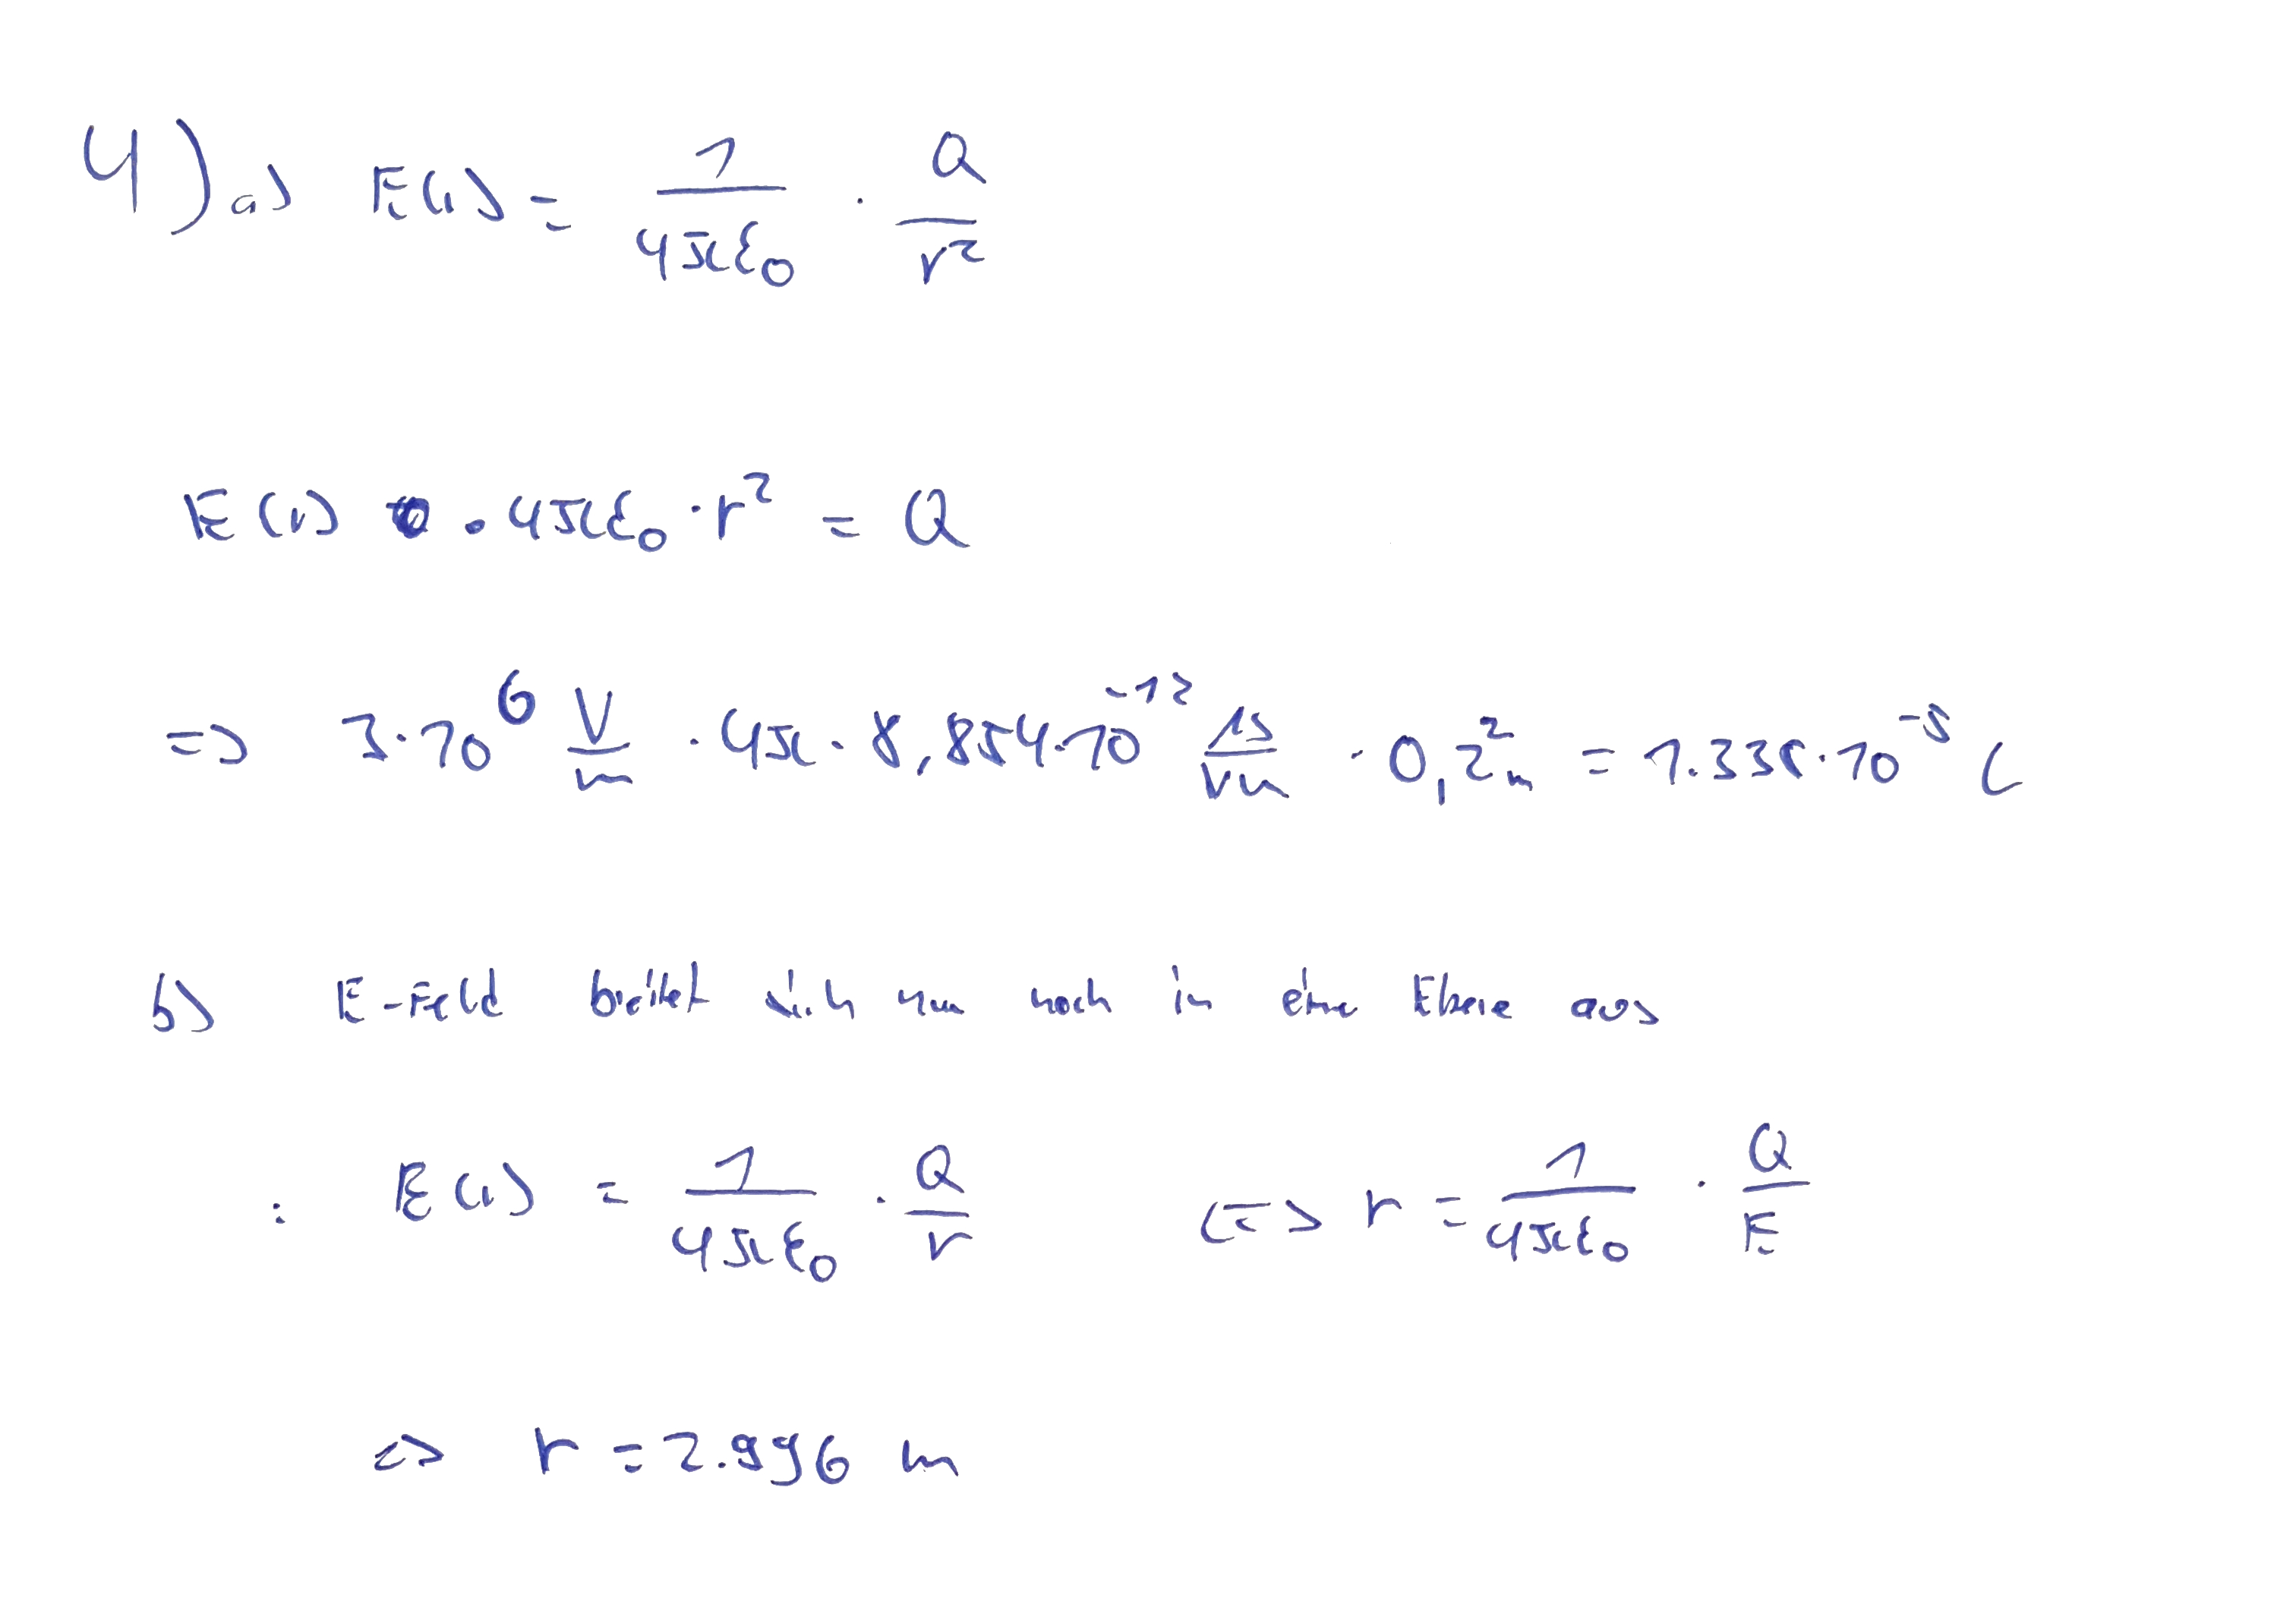
\includegraphics[width=15cm]{4.jpg}


\newpage

\section*{Aufgabe 5}
% ...
\par{a)}
Nabla in Kugelkoordinaten:
\[ \nabla = \er \cdot \delr + \et \cdot \frac{1}{r} \delt + \ep \cdot \frac{1}{r \sin\theta} \delp \]
Die Divergenz eines Radialfeldes $\vec{E}(\vec{r}) = \alpha r^\beta \er$ lautet dadurch:
\begin{align*}
	\vec{\nabla} \cdot \vec{E}(\vec{r}) 
	&= \left(  \er \delr + \et \frac{1}{r} \delt + \ep  \frac{1}{r \sin\theta} \delp \right) \cdot \alpha r^\beta \er \\
	% skalar produkt aufgeloest
	&= \left(\er * \delr (\alpha r^\beta \er )
		+ \et * \frac{1}{r} \delt (\alpha r^\beta \er )
		+ \ep * \frac{1}{r\sin\theta} \delp (\alpha r^\beta \er) \right) \\
	% ableiten
	&= \left(\er \cdot \er \cdot \alpha \beta r^{\beta - 1}
		+ \frac{1}{r} \cdot \et \cdot \et \alpha r^\beta
		+ \frac{1}{r\sin\theta} \cdot \ep \cdot \ep \cdot \alpha r^\beta \right) \\
	% skalarprodukte
	&= \left(\alpha \beta r^{\beta - 1}
		+ \frac{1}{r} \alpha r^\beta
		+ \frac{1}{r\sin\theta}  \alpha r^\beta \right) \\
	% kuerzen
	&= \left( \alpha\beta r^{\beta - 1} +\alpha r^{\beta - 1} +\alpha r^{\beta - 1} \right) \\
	&= \alpha (\beta + 2) r^{\beta - 1}
\end{align*}
Da $\nabla \cdot \vec{E}(\vec{r}) = 1$ für alle $r$ erfüllt sein soll, muss die Gleichung unabhängig von $r$ sein:
\begin{align*}
	\alpha (\beta + 2) r^{\beta - 1} \overset{!}&{=} 1
	\quad \Rightarrow
	\beta = 1 \text{ damit Gleichung unabhängig von r ist}
	\\
	\Leftrightarrow
	\alpha * 3 &= 1 \\
	\Leftrightarrow
	\alpha &= \frac{1}{3} \\
	\Rightarrow \vec{E}(\vec{r}) &= \frac{1}{3} r \hat{e}_r
\end{align*}

\par{b)}
\begin{align*}
	V_{Kugel} 
	&= \iiint dV = \iiint \vec{\nabla} \cdot \vec{E}(\vec{r})dV \overset{\text{Satz v. Gauß}}{=}
	\iint \vec{E}(\vec{r})dA \\
	% einsetzen	
	&= \iint \frac{1}{3} R \hat{e}_r dA \\
	&= \int_0^{2\pi} \int_0^\pi \frac{R}{3} \ \hat{e}_r \cdot \hat{n} * R^2\sin\theta \ d\theta d\varphi \\
	% integral vereinfahen
	&= \frac{R^3}{3} \int_0^{2\pi} \int_0^\pi \sin\theta \ d\theta d\varphi \\
	% integral loesen
	&= \frac{R^2}{3} * 4\pi \\
	&= \frac{4}{3} * \pi * R^3
\end{align*}

\newpage
\section*{Aufgabe 6}
\[
	\vec F (\vec r) = 
	\begin{pmatrix}
		y^3 \\ x^2 \\ z
	\end{pmatrix}
\]

Das Linienintegral in den Teil entlang der x-Achse $r_1$ und entlang der Kreislinie $r_2$ aufteilt werden. Die Parametrisierung lautet dann:
\[
	r_1 = R * \begin{pmatrix} t \\ 0 \\ 0 \end{pmatrix}, \quad 
	t \in [-1, 1] \qquad 
	r_2 = \overline \gamma (t) = R *
		\begin{pmatrix}
			\cos(t) \\ \sin(t) \\ 0
		\end{pmatrix}
		\quad
	t \in [0, \pi ]
\]
Daraus folgt dann das Linienintegral:
\begin{align*}
	\int_{\partial A} \vec F (\vec r ) \cdot d\vec s
	&= \int_{r_1} \vec F (\vec r_1 ) \cdot d\vec r_1 +
	\int_{r_2} \vec F (\vec r_2 ) \cdot d\vec r_2 \\
	% substitution
	&= \int_{-1}^1 \vec F (\vec r_1 ) \cdot \frac{d\vec r_1(t)}{dt} dt +
	\int_0^\pi \vec F (\vec r_2 ) \cdot \frac{d\vec r_2(t)}{dt} dt \\
	&= \int_{-1}^1
	% werte in vektoren einsetzen
	\begin{pmatrix} 0 \\ (R*t)^2 \\ 0 \end{pmatrix}
	\cdot
	\begin{pmatrix} R \\ 0 \\ 0 \end{pmatrix}
	dt + 
	\int_0^\pi
	\begin{pmatrix} R^3 * \sin^3(t) \\ R^2 * \cos^2(t) \\ 0 \end{pmatrix}
	\cdot
	\begin{pmatrix} -R*\sin(t) \\ R*\cos(t) \\ 0 \end{pmatrix}
	dt \\
	% skalarprodukte ausrechnen
	&= \int_{-1}^1 0 \ dt + 
	\int_0^\pi
	\left(
	-R^4 * \sin^4(t) + R^3 * \cos^3(t)
	\right)
	dt \\
	% integral aufteilen
	&= -R^4 \int_0^\pi \sin^4(t) dt + 
	R^3 \underbrace{\int_0^\pi \cos^3(t) dt }_{= 0} \\
	% loesen
	&= -R^4 \int_0^\pi \sin^4(t) dt = -R^4 * \pi * \frac 3 8
\end{align*}
Das Flächen-Integral kann ueber eine Umformung in Zylinderkoodinaten vereinfacht werden:
\begin{align*}
	\iint_{A} \vec \nabla \times \vec F d\vec A &= 
	\iint_{A} \left( \vec \nabla \times \vec F\right) \cdot  \vec e_z \ dA \\
	&= \iint_{A}
	\begin{pmatrix} 0 \\ 0 \\ 2x - 3y^2 \end{pmatrix} \cdot
	\begin{pmatrix} 0 \\ 0 \\ 1 \end{pmatrix} dA \\
	&= \iint_{A} \left( 2x - 3y^2 \right) dA \\
	% umformen in zylinder koordinaten
	&= \int_0^\pi \int_0^R 
	\left(
		2 * \rho * \cos\varphi - 
		3 * (\rho \sin\varphi)^2
	\right) * \rho \
	d\rho d\varphi \\
	% rho integral loesen
	&= \int_0^\pi 
	\left(
		\frac 2 3 R^3 \cos\varphi - 
		\frac 3 4 R^4 \sin^2\varphi
	\right)
	d\varphi \\
	% trennen
	&= 
	\underbrace{\int_0^\pi 
	\left(
		\frac 2 3 R^3 \cos\varphi
	\right)
	d\varphi}_{= 0}
	-
	\int_0^\pi
	\left(
		\frac 3 4 R^4 \sin^2\varphi
	\right)
	d\varphi \\
	% loesen
	&= -R^4 \frac 3 4 \int_0^\pi \sin^2\varphi d\varphi = -R^4 * \pi *
	\frac 3 8
\end{align*}
Die Lösung der Integrale über $\sin^n(t)$ folgt aus der Redduktionsformel.


\end{document}
